\chapter{Three Point Inequalities and Similar Triangles}\label{chap:threepoint}

Every convergence proof for an MM algorithm or an accelerated gradient method
rests, at bottom, on one inequality. It compares the new iterate with an
arbitrary reference point through three distances, and in its Euclidean form
it is nothing more than the law of cosines for the triangle formed by the old
iterate, the new iterate and the reference point. Nesterov's accelerated
method can be organized around it as a sequence of similar triangles, and the
energy that decreases along the iterates is assembled from it. This chapter
works the inequality as hard as it will go. We prove it, use it to derive the
classical rates, and then turn it on the two objects of this book.

On Switching MM it gives something new. A three point argument proves that
on smooth convex functions, which need not be strongly convex, two steps of
Switching MM are worth $2+\beta$ steps of gradient descent rather than two,
provided the long step $1+\beta$ is at most the golden ratio. Performance
estimation then indicates that the resulting rate, after the usual tightening,
is exact: we conjecture that the worst case of Switching MM is $LR^2/((4+2\beta)N+2)$, a factor
$1+\beta/2$ below gradient descent, for every $\beta$ up to a threshold
$\beta_2=0.686$ that we compute in closed form. Every step momentum at the Collatz value of
$\beta$ is worse than gradient descent in the worst case for $4\le N\le15$ and only slightly better for $16\le N\le20$, so on this
measure the parity schedule wins. Acceleration in the sense of a $1/N^2$
rate requires the similar triangles, and we show that it survives arbitrary
switching with plain gradient steps.

On the Collatz map the answer is half yes. The three point identity holds
exactly, with the book's own majorizer of the logarithm: each step of the
Syracuse map splits into a linear term, which is a martingale in the model,
and a Bregman divergence, which dissipates at least a fixed amount at every
step. What is missing is the other half of the three point inequality, the
optimality of the step, and we explain exactly why it cannot be supplied.

\section{The three point identity and the three point inequality}\label{sec:ch7b:threepoint}

Let $h$ be a differentiable convex function on a convex set, and write
\[
  D_h(a,b)=h(a)-h(b)-\langle\nabla h(b),a-b\rangle\ \ge0
\]
for its Bregman divergence. For $h=\half\|\cdot\|^2$ this is
$\half\|a-b\|^2$; for the negative entropy $h(x)=\sum_ix_i\log x_i$ on the
simplex it is the Kullback and Leibler divergence; for $h=-\log$ on the
positive reals it is the Itakura and Saito divergence
$D(a,b)=a/b-1-\log(a/b)$, which will reappear in \cref{sec:ch7b:collatz}.

\begin{lemma}[Three point identity]\label{lem:ch7b:identity}
For all $u,z,z^+$ in the domain of $h$,
\[
  D_h(u,z)-D_h(u,z^+)-D_h(z^+,z)=\langle\nabla h(z^+)-\nabla h(z),\,u-z^+\rangle.
\]
For $h=\half\|\cdot\|^2$ it reads
$2\langle z-z^+,\,u-z^+\rangle=\|u-z^+\|^2+\|z-z^+\|^2-\|u-z\|^2$, which is
the law of cosines for the triangle with vertices $u$, $z$ and $z^+$.
\end{lemma}

\begin{proof}
Expand the three divergences from the definition. The values $h(u)$, $h(z)$
and $h(z^+)$ cancel in pairs, and the inner products collect to the right
hand side.
\end{proof}

\begin{lemma}[Three point inequality]\label{lem:ch7b:inequality}
Let $\psi$ be convex, let $C$ be a closed convex set, and let
\[
  z^+=\arg\min_{x\in C}\bigl\{\psi(x)+D_h(x,z)\bigr\}.
\]
Then for every $u\in C$,
\[
  \psi(z^+)+D_h(z^+,z)\;\le\;\psi(u)+D_h(u,z)-D_h(u,z^+).
\]
\end{lemma}

\begin{proof}
Since $z^+$ minimizes a convex function over a convex set, there is a
subgradient $\xi\in\partial\psi(z^+)$ with the variational inequality
$\langle\xi+\nabla h(z^+)-\nabla h(z),\,u-z^+\rangle\ge0$ for every $u\in C$.
By convexity $\psi(u)\ge\psi(z^+)+\langle\xi,u-z^+\rangle$. Adding the two
and using \cref{lem:ch7b:identity} for the term in $\nabla h$ gives the claim.
\end{proof}

The proof has two ingredients and it is worth keeping them apart. The first
is the identity, which is pure geometry and holds for any three points. The
second is the variational inequality, which holds because $z^+$ is the
minimizer of a convex function over a convex set. The identity is
bookkeeping; the variational inequality is where the information enters.
\Cref{fig:ch7b:geometry}(a) shows the Euclidean case: the step from $z$ to
$z^+$ is a move against a gradient, and the inequality says that the angle at
$z^+$ in the triangle $(u,z,z^+)$ is not acute in the direction that would let
$z^+$ drift away from $u$.

\begin{figure}[t]
\centering
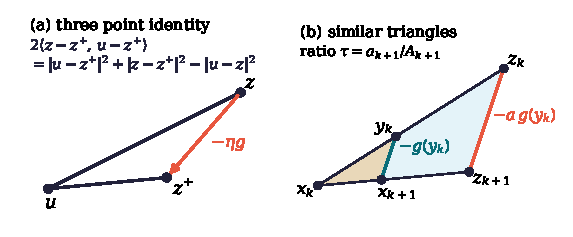
\includegraphics[width=\textwidth]{figures/ch5d_geometry.pdf}
\caption{(a) The three point identity is the law of cosines for the triangle
formed by a reference point $u$, an iterate $z$ and the next iterate $z^+$. (b)
The method of similar triangles: the gradient point $y_k$ and the new iterate
$x_{k+1}$ are the images of $z_k$ and $z_{k+1}$ under the homothety with centre
$x_k$ and ratio $\tau=a_{k+1}/A_{k+1}$, so the two shaded triangles are
similar.}
\label{fig:ch7b:geometry}
\end{figure}

\section{MM convergence from the inequality}\label{sec:ch7b:mm}

Let $f$ be convex and $L$ smooth relative to $h$, in the sense of Bauschke,
Bolte and Teboulle~\cite{bauschke2017} and Lu, Freund and
Nesterov~\cite{lu2018}:
\[
  f(x)\le f(z)+\langle\nabla f(z),x-z\rangle+L\,D_h(x,z)\qquad\text{for all }x,z.
\]
The right hand side, as a function of $x$, is a majorizer\index{majorization} of $f$ that touches
it at $z$, and minimizing it is an MM step\index{MM algorithm}. For $h=\half\|\cdot\|^2$ the
condition is ordinary $L$ smoothness and the MM step is the gradient step
$z^+=z-\nabla f(z)/L$; for the entropy on the simplex it is the exponentiated
gradient update.

\begin{theorem}[MM rate from the three point inequality]\label{thm:ch7b:mm}
Let
\[
  z_{k+1}=\arg\min_{x\in C}\{f(z_k)+\langle\nabla f(z_k),x-z_k\rangle+LD_h(x,z_k)\}.
\]
Then for every $u\in C$ and every $k\ge1$,
\[
  f(z_k)-f(u)\;\le\;\frac{L\,D_h(u,z_0)}{k}.
\]
\end{theorem}

\begin{proof}
Apply \cref{lem:ch7b:inequality} with $\psi(x)=\langle\nabla f(z_k),x\rangle/L$:
\begin{multline*}
  \langle\nabla f(z_k),z_{k+1}\rangle+L\,D_h(z_{k+1},z_k)\\
  \le\langle\nabla f(z_k),u\rangle+L\,D_h(u,z_k)-L\,D_h(u,z_{k+1}).
\end{multline*}
Relative smoothness bounds $f(z_{k+1})$ by $f(z_k)$ plus the left hand side
minus $\langle\nabla f(z_k),z_k\rangle$, and convexity bounds
$f(z_k)+\langle\nabla f(z_k),u-z_k\rangle$ by $f(u)$. Together,
$f(z_{k+1})-f(u)\le L\,D_h(u,z_k)-L\,D_h(u,z_{k+1})$. Summing over the first
$k$ steps telescopes the right hand side, and since the MM step never
increases $f$, the left hand side is at least $k(f(z_k)-f(u))$.
\end{proof}

For gradient descent this is the familiar bound $LR^2/(2k)$ with
$R=\|z_0-x_*\|$. It is not tight: the exact worst case, found by Drori and
Teboulle~\cite{drori2014} by performance estimation\index{performance estimation}, is $LR^2/(4k+2)$. The factor
two is what a cleverer combination of the same inequalities gains, and we will
meet it again.

\section{Similar triangles and acceleration}\label{sec:ch7b:triangles}

Acceleration keeps the three point inequality and changes what it is
applied to. Nesterov's method in the form of the \emph{method of similar
triangles} of Gasnikov and Nesterov~\cite{gasnikov2018} runs three sequences.
Start from $x_0=z_0$ and $A_0=0$. At step $k$ choose $a_{k+1}>0$ with
$L\,a_{k+1}^2=A_{k+1}$, where $A_{k+1}=A_k+a_{k+1}$, and set
\begin{gather*}
  y_k=\frac{A_kx_k+a_{k+1}z_k}{A_{k+1}},\qquad
  z_{k+1}=z_k-a_{k+1}\nabla f(y_k),\\
  x_{k+1}=\frac{A_kx_k+a_{k+1}z_{k+1}}{A_{k+1}}=y_k-\frac1L\nabla f(y_k).
\end{gather*}
The point $y_k$ divides the segment from $x_k$ to $z_k$ in the ratio
$\tau=a_{k+1}/A_{k+1}$, and $x_{k+1}$ divides the segment from $x_k$ to $z_{k+1}$
in the same ratio, so the triangle $(x_k,y_k,x_{k+1})$ is the image of
$(x_k,z_k,z_{k+1})$ under a homothety with centre $x_k$
(\cref{fig:ch7b:geometry}(b)). The $z$ sequence takes long steps with growing
weights $a_{k+1}$; the $x$ sequence takes ordinary gradient steps from the
points $y_k$; the similar triangles tie them together. The form
$x_{k+1}=y_k-\nabla f(y_k)/L$ follows from
$x_{k+1}-y_k=\tau(z_{k+1}-z_k)=-\tau a_{k+1}\nabla f(y_k)$ and
$\tau a_{k+1}=a_{k+1}^2/A_{k+1}=1/L$.

\begin{theorem}[The energy of similar triangles]\label{thm:ch7b:triangles}
Let $f$ be convex and $L$ smooth with a minimizer $x_*$, and put
\[
  E_k=A_k\bigl(f(x_k)-f_*\bigr)+\half\|z_k-x_*\|^2.
\]
Then $E_{k+1}\le E_k$ for every $k$, and $A_k\ge k^2/(4L)$, so that
\[
  f(x_k)-f_*\;\le\;\frac{2L\|x_0-x_*\|^2}{k^2}.
\]
\end{theorem}

\begin{proof}
Write $g=\nabla f(y_k)$, $A=A_k$, $A'=A_{k+1}$, $a=a_{k+1}$. The $z$ step is the
minimizer of $a\langle g,x\rangle+\half\|x-z_k\|^2$, so \cref{lem:ch7b:inequality}
with $u=x_*$ gives
\begin{equation}\label{eq:ch7b:zstep}
  a\langle g,z_{k+1}-x_*\rangle\le\half\|x_*-z_k\|^2-\half\|x_*-z_{k+1}\|^2-\half\|z_{k+1}-z_k\|^2.
\end{equation}
The descent lemma at $y_k$, with $x_{k+1}-y_k=(a/A')(z_{k+1}-z_k)$ and
$La^2=A'$, gives
\[
  A'f(x_{k+1})\le A'f(y_k)+a\langle g,z_{k+1}-z_k\rangle+\half\|z_{k+1}-z_k\|^2.
\]
Split $a\langle g,z_{k+1}-z_k\rangle=a\langle g,z_{k+1}-x_*\rangle+a\langle g,x_*-z_k\rangle$
and use \eqref{eq:ch7b:zstep} on the first part; the terms in
$\|z_{k+1}-z_k\|^2$ cancel. Because $A'y_k=Ax_k+az_k$,
\begin{align*}
  A'f(y_k)+a\langle g,x_*-z_k\rangle
  &=A\bigl(f(y_k)+\langle g,x_k-y_k\rangle\bigr)\\
  &\qquad+a\bigl(f(y_k)+\langle g,x_*-y_k\rangle\bigr)\\
  &\le Af(x_k)+af_*
\end{align*}
by convexity. Collecting,
\[
  A'f(x_{k+1})\le Af(x_k)+af_*+\half\|z_k-x_*\|^2-\half\|z_{k+1}-x_*\|^2,
\]
and subtracting $A'f_*$ from both sides gives $E_{k+1}\le E_k$. For the growth,
$A'-A=a=\sqrt{A'/L}$, so $\sqrt{A'}-\sqrt A=\sqrt{A'}/(\sqrt L(\sqrt{A'}+\sqrt A))\ge1/(2\sqrt L)$,
and $A_k\ge k^2/(4L)$. Finally $A_k(f(x_k)-f_*)\le E_k\le E_0=\half\|x_0-x_*\|^2$.
\end{proof}

The one place where the triangles are used is the identity $A'y_k=Ax_k+az_k$,
which makes the cross terms cancel exactly. That is the sense in which the
triangle closes. And the one place where acceleration comes from is the
growth of the weights: in \cref{thm:ch7b:mm} the weight of $f(z_k)-f(u)$
increases by one per step, here it increases by $a_{k+1}\approx k/(2L)$, which
is why the rate improves from $1/k$ to $1/k^2$. In momentum form the method
is Nesterov's, with the momentum coefficient $\gamma_k=\tau_{k+1}(1-\tau_k)/\tau_k$ tending to one like
$1-3/k$; the version with a prox step is the algorithm of Beck and
Teboulle~\cite{beck2009}, and Tseng~\cite{tseng2008} gives a unified treatment
of the variants.

\section{Switching MM through the three point lens}\label{sec:ch7b:smm}

Switching MM uses a fixed momentum $\beta$, so its energy weights cannot grow
and no $1/N^2$ rate is possible: on the Huber function of \cref{prop:ch16:lower} the gap after an even number $N$ of steps is $LR^2/((4+2\beta)N+2)$. The right question is what the parity
schedule does to the constant. By \cref{lem:ch6:ystep}, on any differentiable
function a pair of iterations of \smmdet\ from an even iterate $x_{2j}$ is a
long gradient step followed by a unit one,
\[
  y=x_{2j}-\frac{1+\beta}{L}\nabla f(x_{2j}),\qquad x_{2j+2}=y-\frac1L\nabla f(y),
\]
at the cost of two gradient evaluations. Write $s=1+\beta$ and
$\varphi=(1+\sqrt5)/2$ for the golden ratio.

\begin{theorem}[A convex rate for Switching MM]\label{thm:ch7b:smmrate}
Let $f$ be convex and $L$ smooth with a minimizer $x_*$, let
$0\le\beta\le\varphi-1$, and let $R=\|x_0-x_*\|$. Then for every $j$,
\begin{equation}\label{eq:ch7b:pair}
  (2+\beta)\bigl(f(x_{2j+2})-f_*\bigr)\le\frac L2\Bigl(\|x_{2j}-x_*\|^2-\|x_{2j+2}-x_*\|^2\Bigr),
\end{equation}
and consequently, for every even $N$,
\[
  f(x_N)-f_*\;\le\;\frac{LR^2}{(2+\beta)\,N}.
\]
\end{theorem}

\begin{proof}
Write $x_0$, $y$, $x_2$ for one pair and $g_0=\nabla f(x_0)$. The unit step
from $y$ satisfies the three point bound of \cref{thm:ch7b:mm},
\begin{equation}\label{eq:ch7b:unit}
  f(x_2)-f_*\le\frac L2\bigl(\|y-x_*\|^2-\|x_2-x_*\|^2\bigr).
\end{equation}
For the long step, expand the square and use the cocoercivity inequality
$\langle g_0,x_0-x_*\rangle\ge f(x_0)-f_*+\|g_0\|^2/(2L)$:
\[
  \|y-x_*\|^2\le\|x_0-x_*\|^2-\frac{2s}L\bigl(f(x_0)-f_*\bigr)+\frac{s(s-1)}{L^2}\|g_0\|^2.
\]
The descent lemma along the two steps gives
$f(x_0)\ge f(x_2)+s(2-s)\|g_0\|^2/(2L)$. Substituting,
\[
  \|y-x_*\|^2\le\|x_0-x_*\|^2-\frac{2s}L\bigl(f(x_2)-f_*\bigr)+\frac{s(s^2-s-1)}{L^2}\|g_0\|^2.
\]
The last coefficient is nonpositive exactly when $s\le\varphi$, that is
$\beta\le\varphi-1$. Dropping it and inserting the result in \eqref{eq:ch7b:unit}
gives $(1+s)(f(x_2)-f_*)\le\frac L2(\|x_0-x_*\|^2-\|x_2-x_*\|^2)$, which is
\eqref{eq:ch7b:pair} since $1+s=2+\beta$. Summing over $N/2$ pairs telescopes
the right hand side to at most $LR^2/2$, and since both steps decrease $f$, the
left hand side is at least $(N/2)(2+\beta)(f(x_N)-f_*)$.
\end{proof}

The same argument applied to gradient descent gives $LR^2/(2N)$, so the
theorem says that the pair of steps of Switching MM does the work of $2+\beta$
gradient steps. The long step is worth $1+\beta$ unit steps, not merely one,
as long as its overshoot, measured by the term $s(s^2-s-1)\|g_0\|^2$, is paid
for by the decrease of $f$. That is the role of the golden ratio. At the
Collatz value the long step is $s=\lt=1.585$, just inside $\varphi=1.618$. We
know of no reason for the proximity and regard it as a coincidence of the kind
the preface warns against.

\paragraph{The exact worst case.} \Cref{thm:ch7b:smmrate} is loose by the same
factor two as the elementary bound for gradient descent. Performance
estimation\index{performance estimation} computes the exact worst case. For a method that evaluates
gradients at points $p_k=x_0-\sum_{j<k}H_{kj}\nabla f(p_j)$, the largest value of
$f(p_N)-f_*$ over all convex $L$ smooth functions with $\|x_0-x_*\|\le R$ is the
value of a semidefinite program, by the interpolation theorem of Taylor,
Hendrickx and Glineur~\cite{taylor2017}. We solved it for gradient descent,
\smmdet, every step Nesterov with constant $\beta=0.585$ and $0.9$, the method
of similar triangles, and the switched variant of \cref{sec:ch7b:switching}
(scripts \texttt{ch5d\_pep.py} and, for $N=40$, \texttt{ch5d\_cross.py}). \Cref{tab:ch7b:pep} and
\cref{fig:ch7b:pep}(a) give the results. Gradient descent reproduces the
Drori and Teboulle value $1/(4N+2)$ to solver precision, which validates the
computation, and Switching MM matches a formula of the same shape.

\begin{table}[t]
\centering\small
\setlength{\tabcolsep}{3.5pt}
\caption{Exact worst case of $(f(x_N)-f_*)/(LR^2)$ on smooth convex functions,
by performance estimation. Switching MM agrees with $1/((4+2\beta)N+2)$ in
every digit shown. Nesterov's method was not computed at $N=40$.}
\label{tab:ch7b:pep}
\begin{tabular}{@{}rllllll@{}}
\toprule
$N$ & gradient & Switching & Nesterov & Nesterov & switched & similar \\
 & descent & MM & $\beta=0.585$ & $\beta=0.9$ & triangles & triangles \\
\midrule
$2$ & $0.1000$ & $0.0810$ & $0.0810$ & $0.1350$ & $0.1000$ & $0.1000$ \\
$4$ & $0.0556$ & $0.0441$ & $0.0634$ & $0.2434$ & $0.0644$ & $0.0468$ \\
$8$ & $0.0294$ & $0.0231$ & $0.0337$ & $0.2341$ & $0.0335$ & $0.0176$ \\
$12$ & $0.0200$ & $0.0156$ & $0.0209$ & $0.1956$ & $0.0207$ & $0.0091$ \\
$16$ & $0.0152$ & $0.0118$ & $0.0149$ & $0.1616$ & $0.0141$ & $0.0056$ \\
$20$ & $0.0122$ & $0.0095$ & $0.0116$ & $0.1345$ & $0.0102$ & $0.0038$ \\
$40$ & $0.0062$ & $0.0048$ & -- & -- & $0.0034$ & $0.0011$ \\
\bottomrule
\end{tabular}
\end{table}

\begin{conjecture}[The exact convex rate of Switching MM]\label{conj:ch7b:tight}
Let $\beta_2=(\sqrt{33}-3)/4=0.68614\ldots$ be the positive root of $2\beta^3+5\beta^2-3=0$. For
$0\le\beta\le\beta_2$ and every even $N$, the worst case of \smmdet\ over
convex $L$ smooth functions with $\|x_0-x_*\|\le R$ is
\[
  \sup\bigl(f(x_N)-f_*\bigr)=\frac{LR^2}{(4+2\beta)N+2}.
\]
\end{conjecture}

The evidence is the following. For seven values of $\beta$ in $[0,0.64]$,
including the Collatz value, the performance estimation value agrees with the
formula to a relative error below $10^{-7}$ at $N=2,4,8,12,16,20,24,30$, and at
the Collatz value it also agrees at every even $N\le20$ and at
$N=28,32,36,40$ (scripts \texttt{ch5d\_golden.py} and \texttt{ch5d\_cross.py}). At $\beta=0$ the conjecture is the theorem of Drori
and Teboulle. Above $\beta_2$ the formula fails at $N=2$, where the worst case
becomes, numerically, $\beta^2LR^2/6$ (\cref{prop:ch16:lower} proves it is at least this); the two expressions cross where $\beta^2(10+4\beta)=6$,
which is the cubic above. The interpretation is an overshoot followed by one
plain step: the long step can carry the iterate past the minimizer by a
fraction $\beta$ of the distance, and $1/6$ is the one step worst case of
gradient descent. The failure at larger $N$ sets in later: the formula holds numerically
at $N=4$ up to $\beta=0.838$ and at $N=6$ up to $0.891$
(\cref{fig:ch7b:pep}(b)), so $N=2$ appears to be the binding case and the formula should hold
for all even $N$ exactly when $\beta\le\beta_2$. For $\beta$ between $\beta_2$ and
one it appears to hold once $N$ is large enough (\cref{conj:ch16:full}). \Cref{sec:ch16:p11} completes the picture: it gives the
second branch, conjecturally, in closed form for every $\beta<1$, explicit worst functions for
both branches, and a proof of the conjecture for $N=4$, and for $N=2$ when $\beta\le0.6446$.

\begin{figure}[t]
\centering
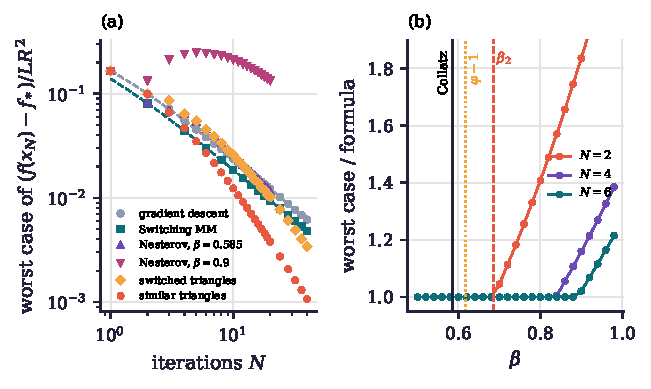
\includegraphics[width=\textwidth]{figures/ch5d_pep.pdf}
\caption{(a) Exact worst cases on smooth convex functions. Dashed lines:
$1/(4N+2)$ for gradient descent and $1/((4+2\beta)N+2)$ for Switching MM. Every
step Nesterov at $\beta=0.9$ has a large transient; similar triangles decay like
$1/N^2$, and the switched version overtakes Switching MM near $N=24$. (b) Worst
case of Switching MM divided by the conjectured formula, against $\beta$, for
$N=2,4,6$. Numerically the formula is exact up to $\beta_2$; the golden threshold of
\cref{thm:ch7b:smmrate} and the Collatz value are marked.}
\label{fig:ch7b:pep}
\end{figure}

Three things follow from the table. First, the ratio of the worst cases of
gradient descent and Switching MM tends to $1+\beta/2=1.29$, the same factor as
in \cref{thm:ch7b:smmrate}: the elementary three point proof captures the
right constant ratio, and only the common factor two is lost. Second, every
step Nesterov at the same $\beta=0.585$ is worse than gradient descent in the
worst case for $4\le N\le15$ and only slightly better for $16\le N\le20$, while Switching MM
is better at every even $N\ge2$, so on this measure the parity schedule is the better
way to spend a fixed momentum. This
is the reverse of the ordering in the average case experiments on random
quadratics of \cref{sec:ch7:experiments}, where every step injection was
faster; worst case and typical case answer different questions. Third, the
machine learning default $\beta=0.9$ has a worst case that rises to $0.251$ at
$N=5$ and is still eleven times that of gradient descent at $N=20$. Its transient
is the convex counterpart of the noise amplification $1/(1-\beta)=10$ of
\cref{chap:noise}.

In the language of long step gradient methods, Switching MM is a periodic step
size schedule $(1+\beta,1)$. Grimmer~\cite{grimmer2023} and Altschuler and
Parrilo~\cite{altschuler2024} showed that periodic and recursive long step
schedules beat gradient descent's constant and even its rate. The schedule of
Switching MM is the simplest member of that family, and
\cref{conj:ch7b:tight} would give its exact constant.

\section{Acceleration survives switching}\label{sec:ch7b:switching}

The energy of \cref{thm:ch7b:triangles} is robust in a way that matches the
switching results of \cref{chap:difference}.

\begin{proposition}[Every switching rule keeps the energy]\label{prop:ch7b:switch}
Consider any sequence of iterations each of which is either a similar
triangles step, as in \cref{sec:ch7b:triangles}, or a plain gradient step
$x^+=x-(s/L)\nabla f(x)$ with $0<s<2$, which leaves $z$ and $A$ unchanged. The
order of the two kinds of step may be arbitrary and may depend on the
iterates. Then the energy $E=A(f(x)-f_*)+\half\|z-x_*\|^2$ never increases,
and after $J$ similar triangles steps
\[
  f(x)-f_*\;\le\;\frac{2L\|x_0-x_*\|^2}{J^2}.
\]
In particular the switched method that alternates the two kinds of step,
starting with a similar triangles step, satisfies $f(x_N)-f_*\le8L\|x_0-x_*\|^2/N^2$.
\end{proposition}

\begin{proof}
A similar triangles step does not increase $E$ by \cref{thm:ch7b:triangles}.
A plain step with $s<2$ decreases $f$ by the descent lemma and leaves $A\ge0$
and $z$ unchanged, so it does not increase $E$ either. The bound follows from
$A\ge J^2/(4L)$ as before, and for the alternating method $J\ge N/2$.
\end{proof}

This is the convex analogue of \cref{cor:ch5b:anyswitch}, which says that on
quadratics, conditionally on \cref{conj:ch5b:transient}, every switching rule between the two steps of Switching MM is
stable. Here every switching rule between an accelerated step and a plain
one keeps the accelerated rate, measured in accelerated steps. The plain
steps are not wasted in practice, since they decrease $f$, but the energy
gives them no credit. Performance estimation shows that the worst case of the
alternating method approaches the energy bound $\|x_0-x_*\|^2/(2A)$, with $A$ its weight after the $J$ similar triangles steps, from below, reaching $0.72$ of it at
$N=20$ and $0.84$ at $N=40$, that it is no better than Switching MM up to
$N\approx22$, and that it overtakes Switching MM from $N=24$ on, as a $1/N^2$
rate must (\cref{tab:ch7b:pep}). If one wants a parity schedule with acceleration, this
is the way to build it: the momentum must be the shrinking ratio of the similar
triangles, not a fixed $\beta$.

\section{Does something similar happen for the Collatz map?}\label{sec:ch7b:collatz}

We now ask whether the Collatz map has a three point inequality. It has half
of one.

\subsection{The three point identity is exact}

Recall the linear majorizer of the logarithm from \cref{chap:lyapunov},
$\log y'\le\log y+(y'-y)/y$ (\cref{prop:mmdescent}). Its gap is a Bregman
divergence: for $h=-\log$,
\[
  \log y'=\log y+\frac{y'-y}y-D\Bigl(\frac{y'}y\Bigr),\qquad D(t)=t-1-\log t\ \ge0,
\]
and $D(t)=D_h(t,1)$ is the Itakura and Saito divergence~\cite{banerjee2005}.
Apply this along a Syracuse orbit $y_{i+1}=S(y_i)$ and write
$M_i=y_{i+1}/y_i=(3+1/y_i)/2^{k_i}$ with $k_i=\vt(3y_i+1)$.

\begin{proposition}[Bregman decomposition of an orbit]\label{prop:ch7b:bregman}
For every odd $y_0$ and every $N$,
\[
  \log y_N-\log y_0=\sum_{i<N}(M_i-1)\;-\;\sum_{i<N}D(M_i).
\]
Under the stride model of \cref{chap:stochastic}, in which
$M=3/2^k$ with $k$ Geometric$(\half)$, the first sum is a martingale,
$\E M=1$, and the expected dissipation per step equals the drift exactly,
$\E D(M)=-\E\log M=\log(4/3)$.
\end{proposition}

\begin{proof}
The identity is the displayed gap formula summed over the orbit. In the
model $\E M=3\sum_k4^{-k}=1$ and $\E\log M=\log3-2\log2$, so
$\E D(M)=\E M-1-\E\log M=\log(4/3)$.
\end{proof}

This is exactly the structure of the energy proofs above: an increment equal to
a linear term minus a nonnegative divergence. The drift of $\log y$ that the
book has used since \cref{chap:stochastic}, $\log(3/4)$ per Syracuse step, is
in this language minus the expected Bregman dissipation, and the linear term is the additive companion of
the multiplicative martingale of \cref{thm:martingale}, a martingale for the same reason, $\E M=1$. The decomposition holds on real
orbits as well as in the model. Over $400$ orbits from random odd starting
values of $3000$ bits, $2\,898\,459$ Syracuse steps in all, the mean dissipation
per step is $0.28718$ against $\log(4/3)=0.28768$, the mean of $M_i-1$ is
$0.00034$ against $0$, and the variance of $M_i$ is $0.28543$ against the model
value $2/7=0.28571$ (script \texttt{ch5d\_collatz\_bregman.py}).
\Cref{fig:ch7b:collatz}(a) shows the three terms along one orbit: the
martingale part wanders near zero, and the descent of $\log y$ is all
dissipation.

\begin{figure}[t]
\centering
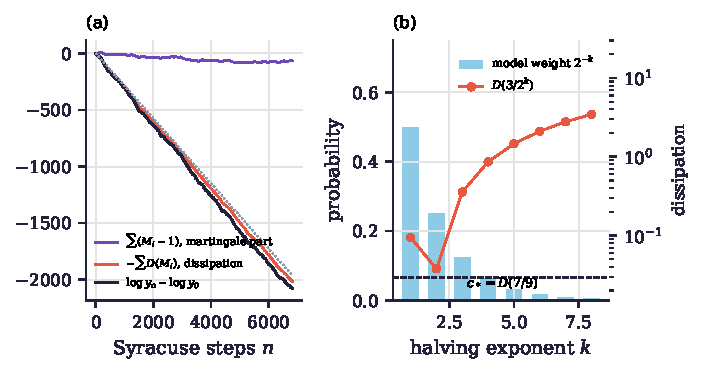
\includegraphics[width=\textwidth]{figures/ch5d_collatz.pdf}
\caption{(a) The Bregman decomposition along the Syracuse orbit of a random
$3000$ bit odd integer: the martingale part $\sum(M_i-1)$, the dissipation
$-\sum D(M_i)$, and their sum $\log y_n-\log y_0$, with the model slope
$-\log(4/3)$ dotted. (b) The dissipation $D(3/2^k)$ of each halving exponent
(log scale, right) and its model weight $2^{-k}$ (left); the dashed line is the
uniform lower bound $c_*$ of \cref{prop:ch7b:dissipation}.}
\label{fig:ch7b:collatz}
\end{figure}

\subsection{Uniform dissipation}

The dissipation is not only positive on average. In the model every multiplier
$3/2^k$ has $D(3/2^k)\ge D(\tfrac34)$, and the real map, with its correction
$1/y$, dissipates a fixed amount at every single step as well.

\begin{proposition}[Uniform dissipation]\label{prop:ch7b:dissipation}
For every odd $y\ge3$,
\[
  D\Bigl(\frac{S(y)}y\Bigr)\;\ge\;c_*=D\bigl(\tfrac79\bigr)=\log\tfrac97-\tfrac29=0.029092\ldots,
\]
with equality only at $y=9$, and $\liminf_{y\to\infty}D(S(y)/y)=D(\tfrac34)=\log\tfrac43-\tfrac14=0.037682\ldots$.
\end{proposition}

\begin{proof}
The function $D$ is convex with its minimum $0$ at $t=1$, decreasing on
$(0,1)$ and increasing on $(1,\infty)$. Write $M=(3+1/y)/2^k$. If $k=1$ then
$M>3/2$ and $D(M)>D(3/2)=\half-\log\tfrac32=0.0945$. If $k\ge3$ then
$M\le(3+\tfrac13)/8=\tfrac5{12}$ and $D(M)\ge D(\tfrac5{12})=0.292$. If $k=2$
then $3y+1\equiv4\pmod8$, so $y\equiv1\pmod8$ and $y\ge9$; then
$\tfrac34<M\le(3+\tfrac19)/4=\tfrac79$, and since $D$ decreases on $(0,1)$,
$D(M)\ge D(\tfrac79)$ with equality only at $y=9$. As $y\to\infty$ along
$y\equiv1\pmod8$ with $k=2$, $M\downarrow\tfrac34$, and the other cases stay
above $D(3/2)>D(3/4)$.
\end{proof}

\begin{corollary}[The martingale part must outrun the dissipation]\label{cor:ch7b:outrun}
If the Syracuse orbit of $y_0$ is unbounded, then
\[
  \limsup_{N\to\infty}\frac1N\sum_{i<N}M_i\;\ge\;1+D(\tfrac34)=1.0377.
\]
If the orbit lies on a nontrivial cycle of $r$ odd elements, then the mean of
the $r$ ratios $M_i$ around the cycle is at least $1+c_*$.
\end{corollary}

\begin{proof}
An unbounded orbit tends to infinity (\cref{lem:ch9:infinity}), so
$D(M_i)\ge D(\tfrac34)-\varepsilon$ for all large $i$, and $\log y_N>\log y_0$
for infinitely many $N$. For those $N$, \cref{prop:ch7b:bregman} gives
$\sum_{i<N}(M_i-1)>\sum_{i<N}D(M_i)$. Dividing by $N$ and letting $\varepsilon\to0$
gives the first claim. On a cycle $\log y_r=\log y_0$, so
$\sum(M_i-1)=\sum D(M_i)\ge rc_*$.
\end{proof}

We should say plainly that these are not new constraints. On a long cycle the
exponents $k_i$ are integers with mean $s/r$ close to $\lt$, and since $2^{-k}$
is convex the mean of $3/2^{k_i}$ is then at least about
$3(3-\lt)/4=1.061$, which is stronger than $1+c_*$; the same convexity argument
applies to divergent orbits through \cref{cor:ch9:freq}. The Bregman
decomposition reorganizes what integrality and the Ces\`aro identity already
give. Its value is that it identifies which term carries the difficulty.

\subsection{What is missing}

The three point inequality of \cref{lem:ch7b:inequality} has two ingredients,
the identity and the variational inequality of a convex minimization. The
Collatz map has the first, exactly, in \cref{prop:ch7b:bregman}, together with
a uniform dissipation that the convex setting supplies only through the term
$D_h(z^+,z)$. It does not have the second. In an MM method the linear term
$\langle\nabla f(z),z^+-u\rangle$ is controlled because $z^+$ was chosen to
minimize the surrogate over a convex set, and the variational inequality
bounds it by the distance terms. In the Collatz map the linear term is
$\sum(M_i-1)$, and nothing controls it: the successor of $y$ is dictated by the
parity of $y$, not chosen to minimize anything. Even if one views the step as a
minimization over a finite set of candidate successors, as in
\cref{chap:mmcollatz}, a finite set carries no variational inequality, and the
three point inequality has nothing to stand on.

In this language the divergence half of the conjecture is a three point
inequality along orbits: for every $y_0$ there is a constant $C(y_0)$ with
\[
  \sum_{i<N}(M_i-1)\;\le\;\sum_{i<N}D(M_i)+C(y_0)\qquad\text{for all }N.
\]
This is equivalent to the boundedness of the orbit, so it is no easier. But it
locates the difficulty precisely. The dissipation is uniform and positive, and
the martingale part is the only term without a sign. In the model it has mean
zero and variance $2/7$ per step, so it grows like $\sqrt N$ while the
dissipation grows like $N$, and the inequality holds with room to spare. Along
one deterministic orbit, controlling the martingale part is the same problem
as controlling the Ces\`aro averages of \cref{chap:divergence}, and it is the
problem no method yet solves.

\section{Summary}\label{sec:ch7b:summary}

\Cref{tab:ch7b:summary} sets the four settings of this chapter side by side.

\begin{table}[ht]
\centering\small
\setlength{\tabcolsep}{3pt}
\caption{The three point structure in four settings.}
\label{tab:ch7b:summary}
\begin{tabular}{@{}>{\raggedright\arraybackslash}p{0.20\textwidth}>{\raggedright\arraybackslash}p{0.17\textwidth}>{\raggedright\arraybackslash}p{0.17\textwidth}>{\raggedright\arraybackslash}p{0.19\textwidth}>{\raggedright\arraybackslash}p{0.19\textwidth}@{}}
\toprule
 & MM step & similar triangles & Switching MM & Collatz map \\
\midrule
three point identity & yes & yes & yes & yes, exactly \\
dissipation & $D_h(z^+,z)$ & $\half\|z^+-z\|^2$, cancelled & cocoercivity & uniform, $c_*=0.029$ \\
optimality of the step & yes & yes & yes, if $1+\beta\le\varphi$ & no \\
growth of the weights & $1$ per step & $\approx k/(2L)$ & $2+\beta$ per pair & none \\
rate & $1/N$ & $1/N^2$ & $1/N$, constant $1+\beta/2$ better & open \\
\bottomrule
\end{tabular}
\end{table}

The three point inequality is the engine of every convergence proof in
convex optimization, and the similar triangles are what make it accelerate.
Pressed on Switching MM it yields a new convex rate with the exact constant
ratio $1+\beta/2$ to gradient descent, a golden ratio condition, and a
conjectured exact worst case that generalizes the theorem of Drori and
Teboulle. Pressed on the Collatz map it yields an exact identity, a uniform
dissipation and a clean statement of what is missing: the optimality of the
step, which a map that does not choose its successor cannot have.

\section*{Notes}

The three point identity for Bregman divergences is due to Chen and
Teboulle~\cite{chen1993}. The method of similar triangles is from Gasnikov and
Nesterov~\cite{gasnikov2018}; Nesterov's method itself is from~\cite{nesterov1983},
the estimate sequence form from~\cite{nesterov2004}, the accelerated proximal
method from Beck and Teboulle~\cite{beck2009}, and a unified analysis of the
variants from Tseng~\cite{tseng2008}. Relative smoothness is due to Bauschke,
Bolte and Teboulle~\cite{bauschke2017} and to Lu, Freund and Nesterov~\cite{lu2018}.
The tight worst case $1/(4N+2)$ of gradient descent is due to Drori and
Teboulle~\cite{drori2014}, and the interpolation conditions behind the
performance estimation programs to Taylor, Hendrickx and Glineur~\cite{taylor2017}.
Long step schedules are studied by Grimmer~\cite{grimmer2023} and by Altschuler
and Parrilo~\cite{altschuler2024}. The Itakura and Saito divergence as a
Bregman divergence is discussed by Banerjee, Merugu, Dhillon and
Ghosh~\cite{banerjee2005}.

\Cref{lem:ch7b:identity}, \cref{lem:ch7b:inequality}, \cref{thm:ch7b:mm} and
\cref{thm:ch7b:triangles} are classical; the proofs are given in the form used
here. \Cref{thm:ch7b:smmrate}, \cref{conj:ch7b:tight} with the threshold
$\beta_2$, \cref{prop:ch7b:switch}, the performance estimation results of
\cref{tab:ch7b:pep}, \cref{prop:ch7b:bregman} in the form stated,
\cref{prop:ch7b:dissipation} and \cref{cor:ch7b:outrun} are new in this book.
\begin{sloppypar}
The scripts are \texttt{ch5d\_pep.py}, \texttt{ch5d\_golden.py},
\texttt{ch5d\_threshold.py}, \texttt{ch5d\_cross.py},
\texttt{ch5d\_collatz\_bregman.py} and \texttt{ch5d\_figures.py}.
\end{sloppypar}

\section*{Exercises}

\begin{exercise}
Prove \cref{lem:ch7b:identity} for a general Bregman divergence, and check that
for $h=-\log$ on the positive reals it gives the identity
$D(a,c)=D(a,b)+D(b,c)+(a-b)(1/c-1/b)$ for the Itakura and Saito divergence
$D(a,b)=a/b-1-\log(a/b)$.
\end{exercise}

\begin{exercise}
Let $h(x)=\sum_ix_i\log x_i$ on the probability simplex. Show that the MM step
of \cref{thm:ch7b:mm} is the exponentiated gradient update
$z^+_i\propto z_i\exp(-\nabla_if(z)/L)$, and state the rate the theorem gives
when $f$ is $L$ smooth relative to the entropy.
\end{exercise}

\begin{exercise}
In the method of similar triangles show that $\tau_k=a_{k+1}/A_{k+1}$ satisfies
$\tau_k\sim2/k$, and that in momentum form $x_{k+1}=y_k-\nabla f(y_k)/L$,
$y_{k+1}=x_{k+1}+\gamma_k(x_{k+1}-x_k)$ the coefficient is
$\gamma_k=\tau_{k+1}(1-\tau_k)/\tau_k$. Compare with Nesterov's $(k-1)/(k+2)$.
\end{exercise}

\begin{exercise}
Show that $s(s^2-s-1)\le0$ for $0<s\le\varphi$ and compute the margin at
$s=\lt$. Then repeat the proof of \cref{thm:ch7b:smmrate} for gradient descent
with a constant step $s/L$, $0<s\le\varphi$, and show that
$f(x_N)-f_*\le LR^2/(2sN)$. Deduce that \eqref{eq:ch7b:pair} is the sum of two one step inequalities, and explain why
\eqref{eq:ch7b:unit}, which treats a step as an MM step, needs $s\le1$.
\end{exercise}

\begin{exercise}
List the odd $y<200$ for which $D(S(y)/y)<D(\tfrac34)$, and explain from the
proof of \cref{prop:ch7b:dissipation} why every one of them is congruent to $1$
modulo $8$.
\end{exercise}
